\section{Introduction}

Speculative bubbles, since at least the early 18th century South Sea Bubble are perceived \footnote{\cite{garber2001famous} pp 127-31 for references, a particularly is \cite{temin2004riding} a case study of a well-informed investor in the South Sea bubble that invested knowingly in the bubble, and found that it was profitable. } to periodically take over markets. %not quite what he says; fundamentals driven then morals story.
The public notoriety of Bitcoin and the massive price increases and their associated publicity  lead to an explosion of attempts to create ``the next bitcoin'' often referred to as ``cryptocurrencies'' or ``coins'', and a vibrant set of exchanges where these are traded, either for each other or money.
The majority of these coins have no viable uses, and their markets would appear driven largely by speculation.
Many of them appear to be nothing but attempts at turning a quick profit from inflating the implied valuation of a coin shortly after creating it.
This is driven by the extremely low cost and effort required to create a new coin, with most being minimal changes to parameters and branding of a pre-existing codebase.
Those who make and trade these coins communicate largely online, and much of their activity is concentrated on public forums, price and volume data from their exchanges is freely available and widely aggregated, and the source code to all coins is public.
This makes cryptocoins an almost ideal window in the social life of a market mania \cite{cosma2008}.
Such study can serve in the computational social sciences a role analogous to that of lesion studies do in neuropsychology.


%\begin{figure}[h!]
%\end{figure}

We present a novel dataset that combines measures derived from the social network in an online forum, market data aggregated over dozens of exchanges, and properties of software implementing hundreds of cryptocoins.
In the forum we identify the introducers of each coin and build measures of their position in the network based on which users have engaged with them threads in the forum before the coin is announced.
We dentify 376 coins that are announced by users of the forum and which can be mapped to price and volume data from exchanges.
From the price and transaction volume data we build measures of the subsequent activity that results from trading in the coin. 
We also asses if coins posibly embody technological inovation based on having more than trivial modifications to previously existing coins sourcecode.

While the mechanisms that drive bubbles have been theoretically  \cite{abolafia1988enacting, earl2007decision, bakker2010social, harras2011grow} and experimentally \cite{moinas2013bubble} in the lab, an exaustive dataset on the social network of those promoting the asset has not been previously available.
While the magnitude of the assets traded is small relative to most financial and commodity markets, it is much larger than even the most lavishly funded experimenter could hope for.
The largest bubble in our dataset, AuroraCoin, reaches a valuation of 1 billon USD on March , with reported daily trading volumes of 6.8M USD, and sheds 90\% of its values in a week, and 99\% of its value in well under a year.
For context, this is equivalent to $1/4$ of Icelands entire foreigh exchange reserves in 2014, \footnote{4.1 Billon USD , The World Bank, Global Economic Monitor, accessed October 2015}, the population of which AuroraCoin promoters claimed they would distribute half of the coins to.

\begin{figure*}
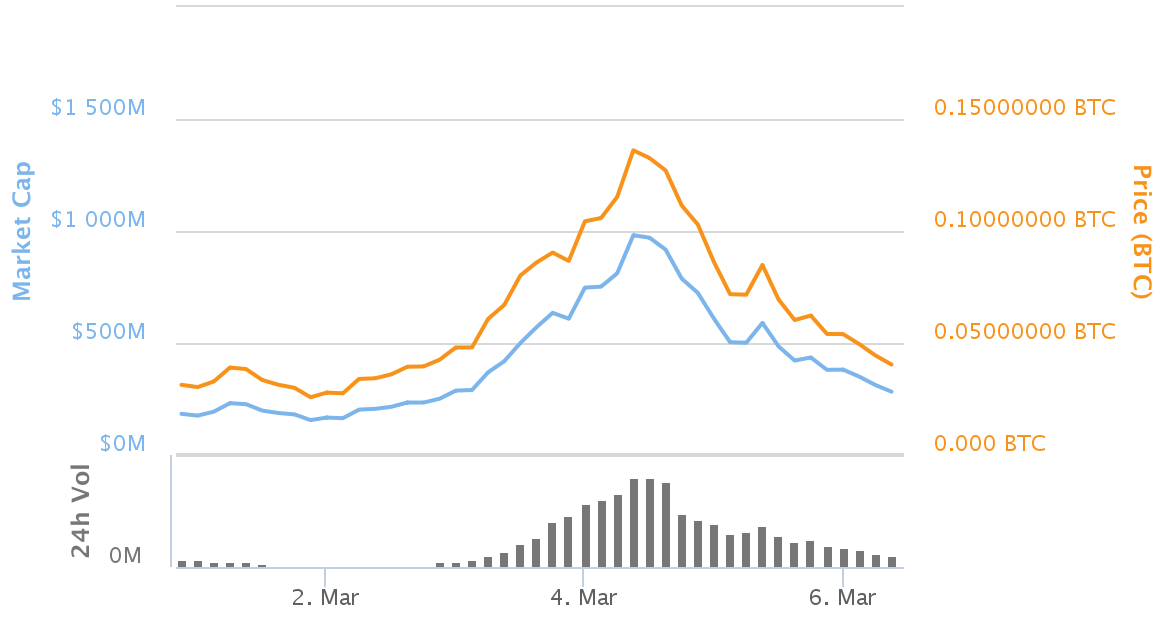
\includegraphics[width=\columnwidth]{AuroraCoin}
\end{figure*}

Using the price and volume data we construct measures of both  the magnitude (how many dollars worth of trading happened in the asset) and the severity of bubbles ( which we define as for each dollar invested at the peak what could be recovered if selling at the volume weighted average prices observed since).
By considering the community structure that exists in the forum before a coin is introduced we are able to predict part of the variation in both the severity and magnitude of the resulting bubble: our best model explains 10\% of the variation in the severity and of the magnitudein our of sample using a penalized linear model and measuring performance out of sample using cross validation. 
The main driver of our explanatory power is the centrality of a user in the directed network derived from the forum.
Both the severity and the magnitude of bubbles increases with the centrality of the user who introduces the coins in the forums.
Interestingly this effect is concentrated in different ways depending on weather the coin software is more than a trivial modification: trivial coins have more severe bubbles the more central their introducers are, while volume is greater the more central the introducer of a nontrivial coin is.


\begin{figure*}
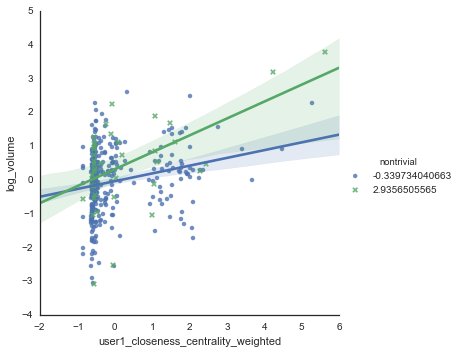
\includegraphics[width=\columnwidth]{volume_centrality}
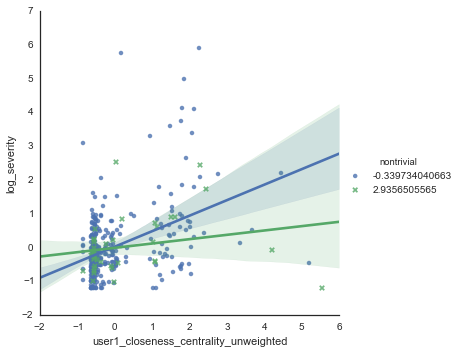
\includegraphics[width=\columnwidth]{severity_centrality}
\end{figure*}

While states can create the demand required for a currency system to run by compelling tax payment in it (for a recent example), non state sponsored currencies must find some other ways of creating demand.
The initial market for which bitcoin has been used (prices denominated in it, transactions only in it) was drug sales.\footnote{A overview of the different drug marketplaces and estimated transaction volumes can be found in \cite{soska2015measuring}. To the best of the authors knowledge no other sector beyond speculation has even remotely substantial volume at present; a very primitive form of unregulated gambling Satoshi Dice, did for a brief pointing the past)   }
Since the cost of producing a new coin is effectively zero, new currencies have thus been floated with every single drug name possible. Many chains can claim to the same name, so exchanges with volume (since speculation is the only possible use of almost all of the coins) become de-facto arbitrators of who has a minimally viable claim.\footnote{While it is theoretically possible to engage in a distributed protocol to exchange between two cryptocurrencies, see part II of lecture 10 in \cite{princeton10}}





%Methodologically the free parameters in the way we do the weights on the weighted graph  is horrible, a millon free parameters get introduced. follow up work for another paper: do some unsupervised feature learning over the dam forums threads to build the network; use some internal validity metric . Find political way of saying this in future work.

